\documentclass{article}
\usepackage[utf8]{inputenc}
\usepackage{enumitem}
\usepackage{mathtools}
\usepackage{float}


\title{Microeconomic Theory HW4 Solutions}
\author{}
\date{November 2022}

\begin{document}

\maketitle

\section*{Exercise 1}
\begin{enumerate}[label=(\alph*)]
\item Andy’s income is given by:
\[m=p_xw_x+p_yw_y=4*20+5*8=120\]
\item Since Andy's utility function is Cobb-Douglas, we use the tangency condition to find Andy’s optimal consumption of goods x and y: 
\[ MRS= \frac{\frac{\partial u}{\partial x}}{\frac{\partial u}{\partial y}}=\frac{y}{2x}= \frac{4}{5}= \frac{p_x}{p_y} \implies y= \frac{8x}{5} \]
By plugging y into the budget constraint $120=4x+5y$ we get Andy’s optimal consumption of goods x and y:
\[ (x^*, y^*)=(10,16)\]
\item Andy is a net seller of good x because:
\[x^*-w_x=10-20<0\]
\item After the price change, Andy's income is given by:
\[m'=p'_xw_x+p_yw_y=10*20+5*8=240\]
\item \[ MRS= \frac{\frac{\partial u}{\partial x}}{\frac{\partial u}{\partial y}}=\frac{y}{2x}= \frac{10}{5}= \frac{p_x}{p_y} \implies y=4x \]
By plugging y into the budget constraint $240=10x+5y$ we get Andy’s optimal consumption of goods x and y after the price change:
\[ (x^*, y^*)=(8,32)\]
\item In the following graph, the budget lines and the optimal consumption found in (b) and (e) are represented:
\begin{figure}[H]
    \centering
    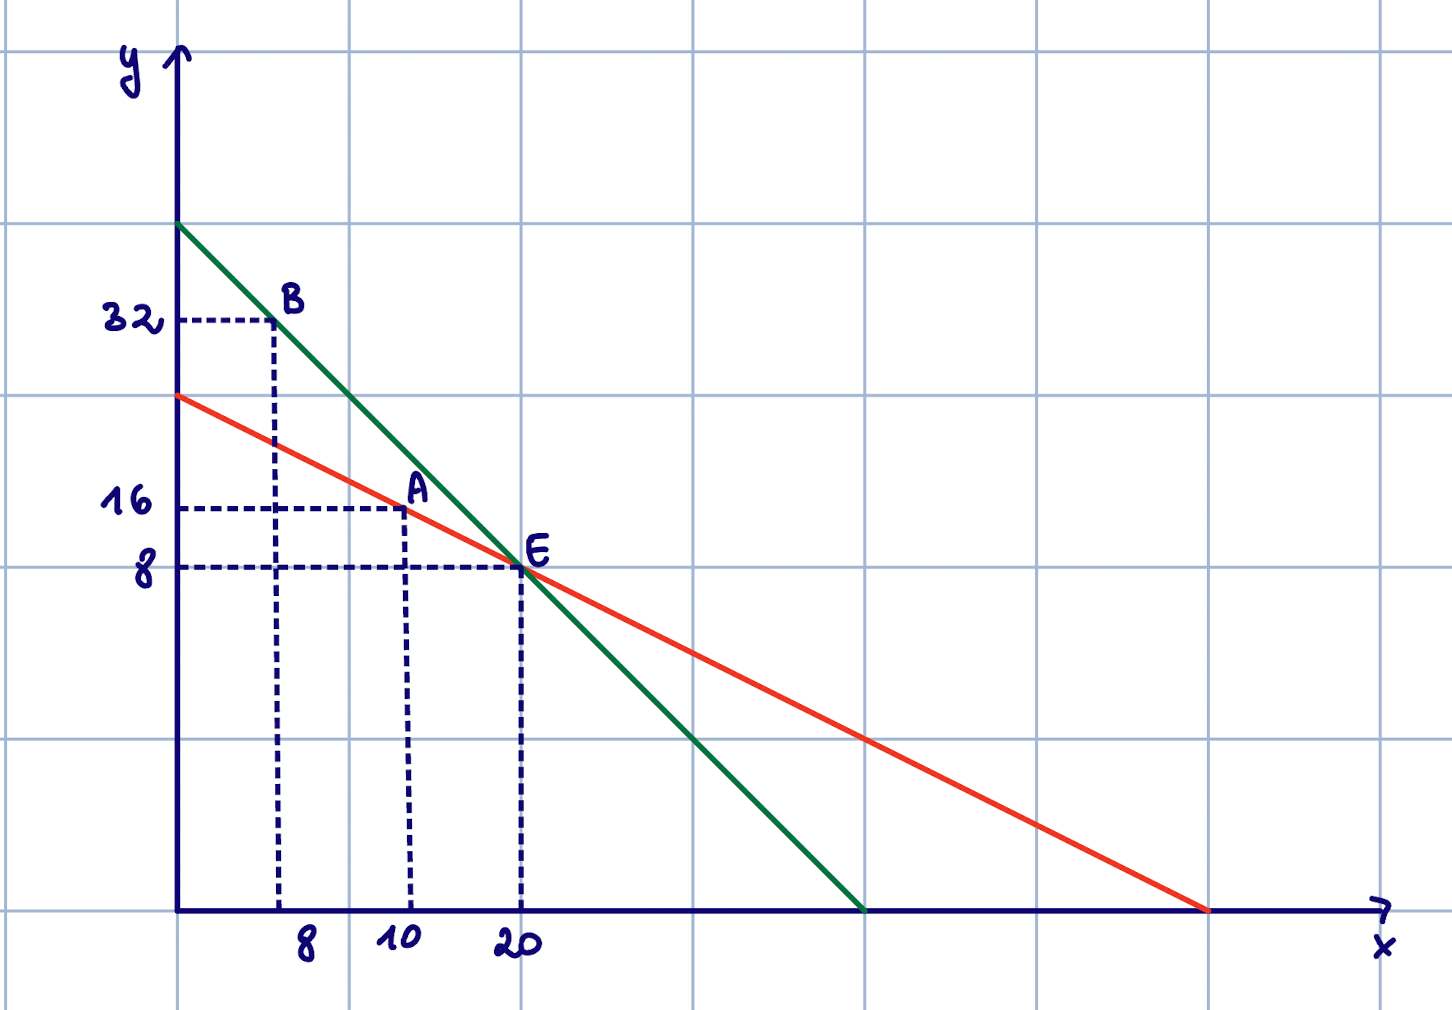
\includegraphics[width=8cm]{fig1.png}
    \caption{}
    \label{fig:galaxy}
\end{figure}
\item Since Andy is a net seller of good x, therefore he is better off when the price of good x increases.
\item \[ p'_xw_x+p_yw_y=10*10+5*16=180\]
\item \[ MRS= \frac{\frac{\partial u}{\partial x}}{\frac{\partial u}{\partial y}}=\frac{y}{2x}= \frac{10}{5}= \frac{p_x}{p_y} \implies y=4x \]
By plugging y into the budget constraint $180=10x+5y$ we get the optimal solution:
\[ (x^*, y^*)=(6,24)\]
The budget line with the same income level before the price change is $10x+5y=120$. The optimal solution is \[(x^*, y^*)=(4,16)\]
The substitution effect is given by 6-10=-4.
The income effect is given by 4-6=-2.
The endowment effect is given by 8-4=4.
\end{enumerate}

\section*{Exercise 2}
\begin{enumerate}[label=(\alph*)]
\item Andy’s income is given by:
\[m=p_xw_x+p_yw_y=12*20+4*10=280\]
\item Since good x and y are perfect complements for Andy, we have:
\[3y=x \implies y= \frac{x}{3} \]
By plugging y into the budget constraint $280=12x+4y$ we get the optimal solution:
\[ (x^*, y^*)=(21,7)\]
\item Andy is a net buyer of x because:
\[x^*-w_x=21-20>0\]
\item After the price change, Andy’s income is given by:
\[m'=p'_xw_x+p_yw_y=2*20+4*10=80\]
\item \[ y =\frac{x}{3} \]
By plugging y into the budget constraint $80=2x+4y$ we get the optimal solution:
\[ (x^*, y^*)=(24,8)\]
\item In the following graph, the budget lines and the optimal consumption found in (b) and (e) are represented:
\begin{figure}[H]
    \centering
    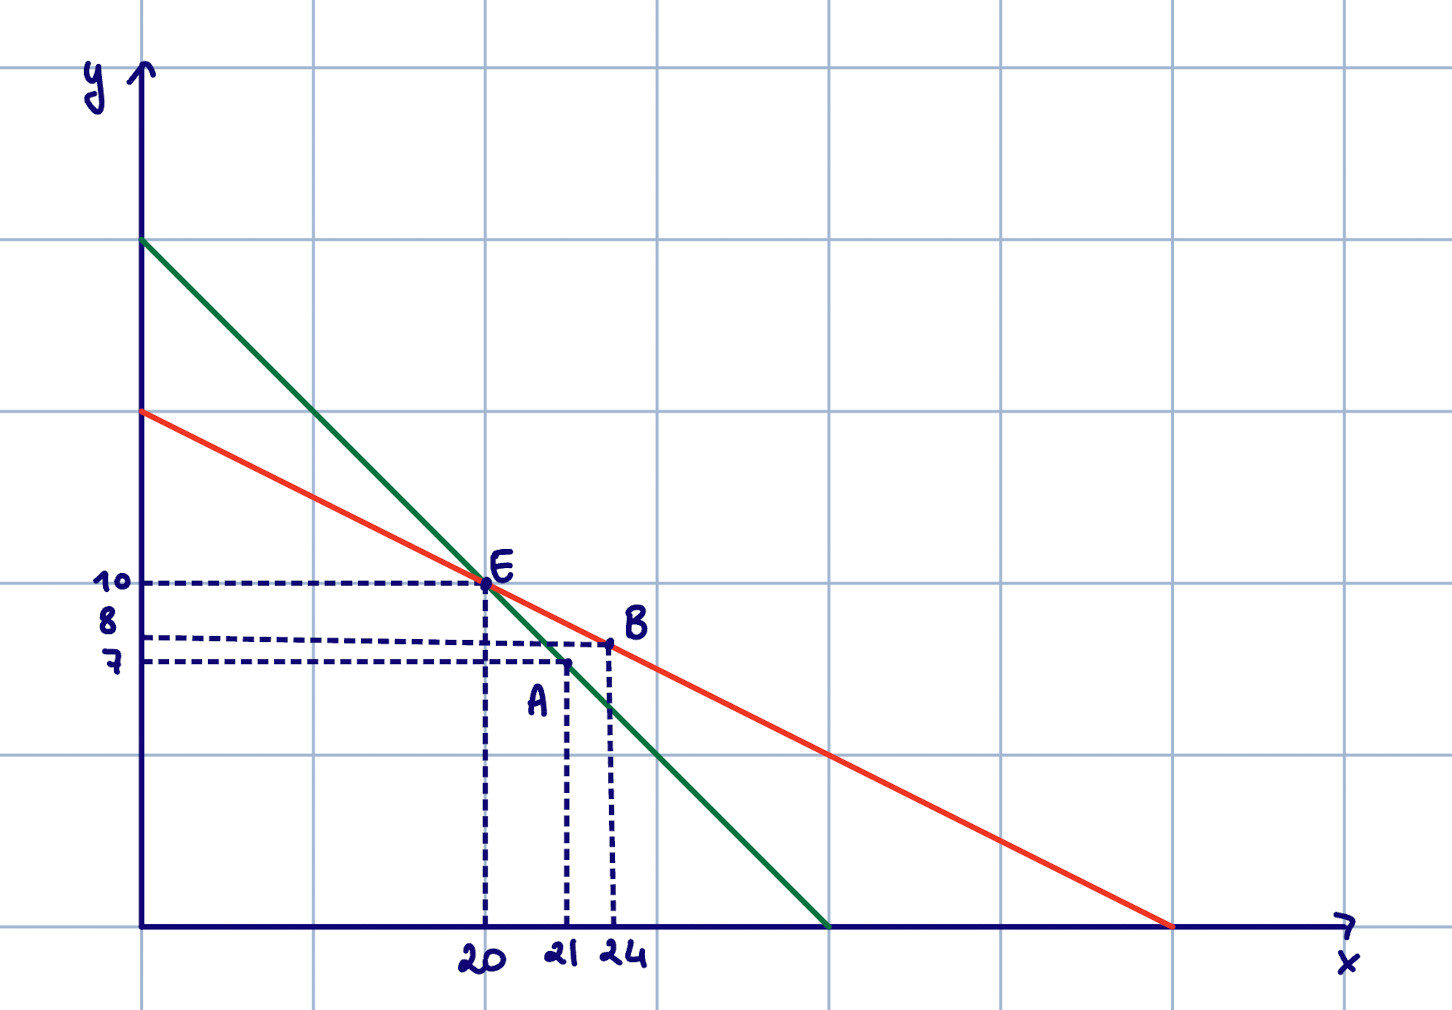
\includegraphics[width=8cm]{fig2.png}
    \caption{}
    \label{fig:galaxy}
\end{figure}
\item Since Andy is a net buyer of good x, therefore he is better off when the price of good x decreases.
\item \[ p'_xw_x+p_yw_y=21*2+7*4=70\]
\item By plugging $y=\frac{x}{3}$ into the budget constraint $70=2x+4y$ we get the optimal solution:
\[ (x^*, y^*)=(21,7)\]
Since the two goods are perfect complements, the substitution effect is zero.
When the budget constraint is given by $280=2x+4y$, $x^*=84$.
The income effect is 84-21=63.
The endowment effect is given by 24-84=-60.
\end{enumerate}

\section*{Exercise 3}
\begin{enumerate}[label=(\alph*)]
\item Andy’s income is given by:
\[m=p_xw_x+p_yw_y=4*20+4*10=120\]
\item Since good x and y are perfect complements for Andy, we have:
\[2y=4x \implies y= \frac{x}{2} \]
By plugging y into the budget constraint $120=4x+4y$ we get the optimal solution:
\[ (x^*, y^*)=(20,10)\]
\item Andy is neither a net buyer nor a net seller of x because:
\[x^*-w_x=0\]
\item \[m'=p'_xw_x+p_yw_y=2*20+4*10=80\]
\item \[ y =\frac{x}{2} \]
By plugging y into the budget constraint $80=2x+4y$ we get the optimal solution:
\[ (x^*, y^*)=(20,10)\]
\item In the following graph, the budget lines and the optimal consumption found in (b) and (e) are represented:

\begin{figure}[H]
    \centering
    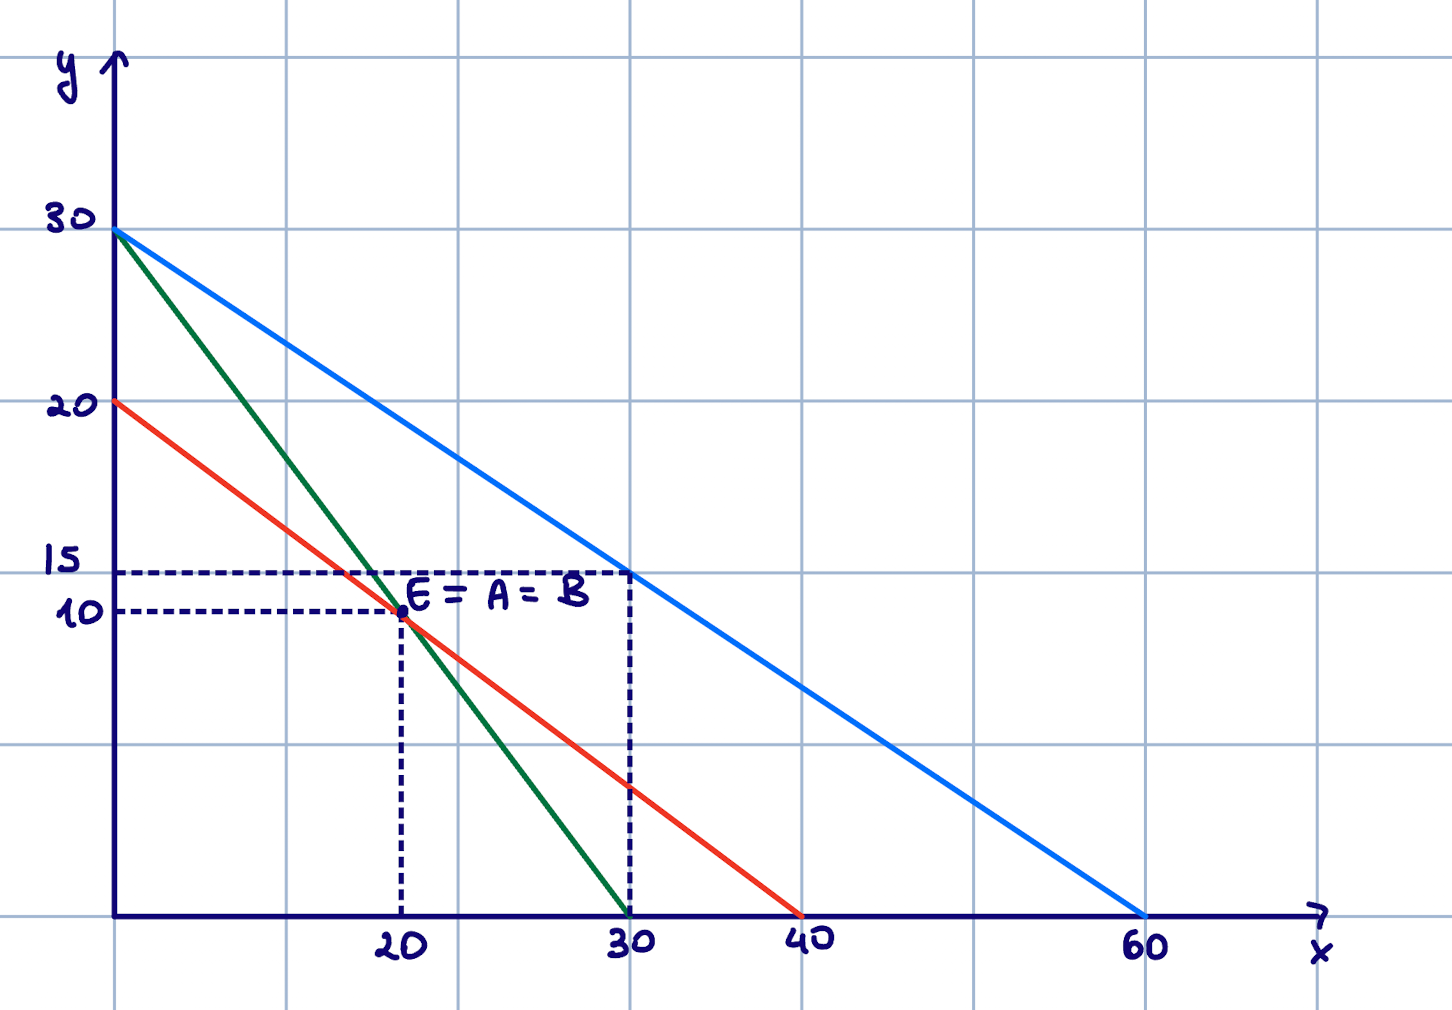
\includegraphics[width=8cm]{fig3.png}
    \caption{}
    \label{fig:galaxy}
\end{figure}
\item Since Andy is neither a net buyer of good x nor a net seller of good x, he is neither better or worse off when the price of good x increases. 
\item \[ p'_xw_x+p_yw_y=2*20+4*10=80\]
\item By plugging $y=\frac{x}{2}$ into the budget constraint $80=2x+4y$ we get the optimal solution:
\[ (x^*, y^*)=(20,10)\]
Since there was no change in demand, the substitution effect, income effect and endowment income effect are all equal to zero. Alternatively, when the budget constraint is given by $120=2x+4y$, $x^*=30$
The income effect is given by $30-20=10$ and the endowment income effect is given by $20-30=-10$. This implies that the two effects offset each other.  
\end{enumerate}

\section*{Exercise 4}
\begin{enumerate}[label=(\alph*)]
\item
\[x_{tot}= x_A+x_B=10+2=12\]
\[y_{tot}= y_A+y_B=2+8=10\]
\item In the following graph, the Edgeworth box is represented:
\begin{figure}[H]
    \centering
    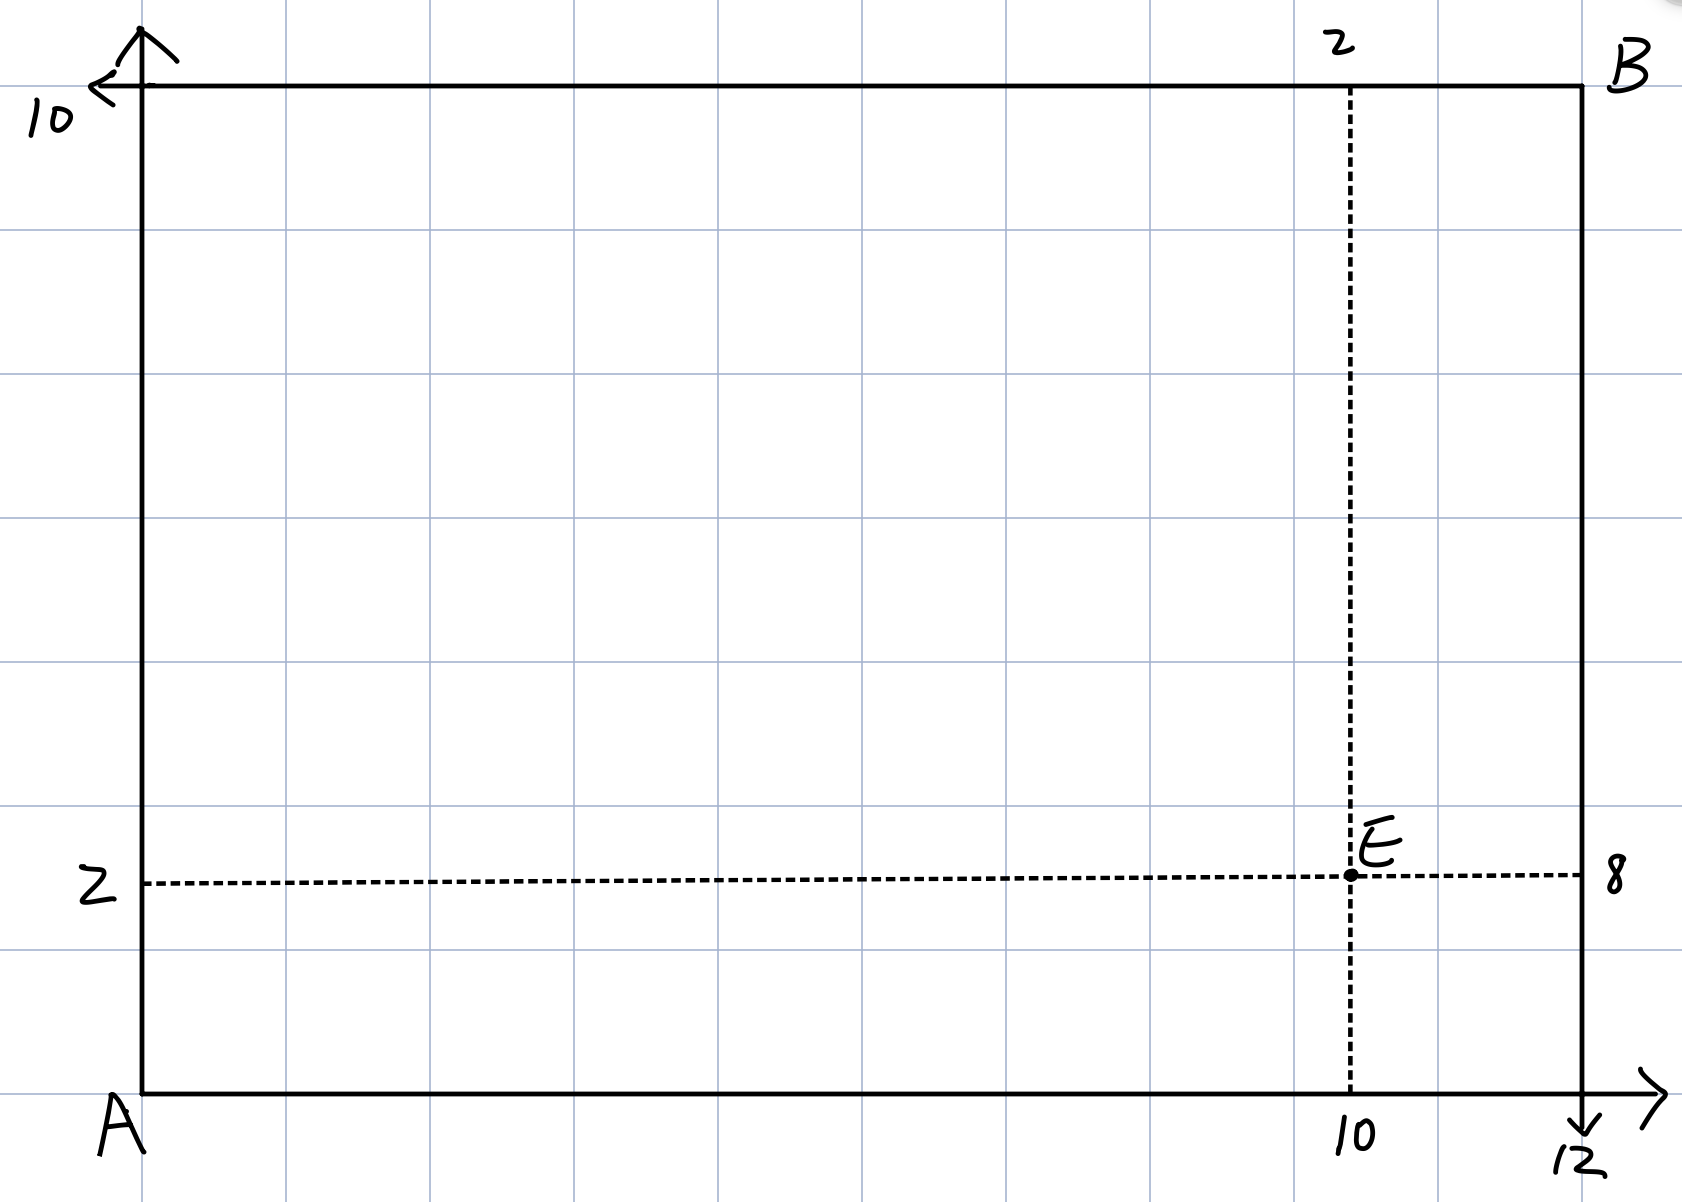
\includegraphics[width=8cm]{fig4.png}
    \caption{Edgeworth Box}
    \label{fig:galaxy}
\end{figure}
\item A bundle is said to be Pareto efficient if there is no way to make someone better off without making someone else worse off. The set of all Pareto efficient bundles constitutes the contract curve.
\item In the case of Cobb-Douglas utility functions, to find the contract curve, we set $MRS_A=MRS_B$: 
\[ MRS_A= \frac{y_A}{2x_A} \]
\[ MRS_B= \frac{y_B}{2x_B}\]
\[\frac{y_A}{2x_A}=\frac{y_B}{2x_B}\]
Since $x_A+x_B=12$ and $x_A+x_B=10$, we can write:
\[\frac{y_A}{x_A}=\frac{y_B}{x_B}=\frac{10-y_A}{12-x_A}\]
\[x_A(10-y_A)=y_A(12-x_A) \implies y_A=\frac{5x_A}{6}\]
\begin{figure}[H]
    \centering
    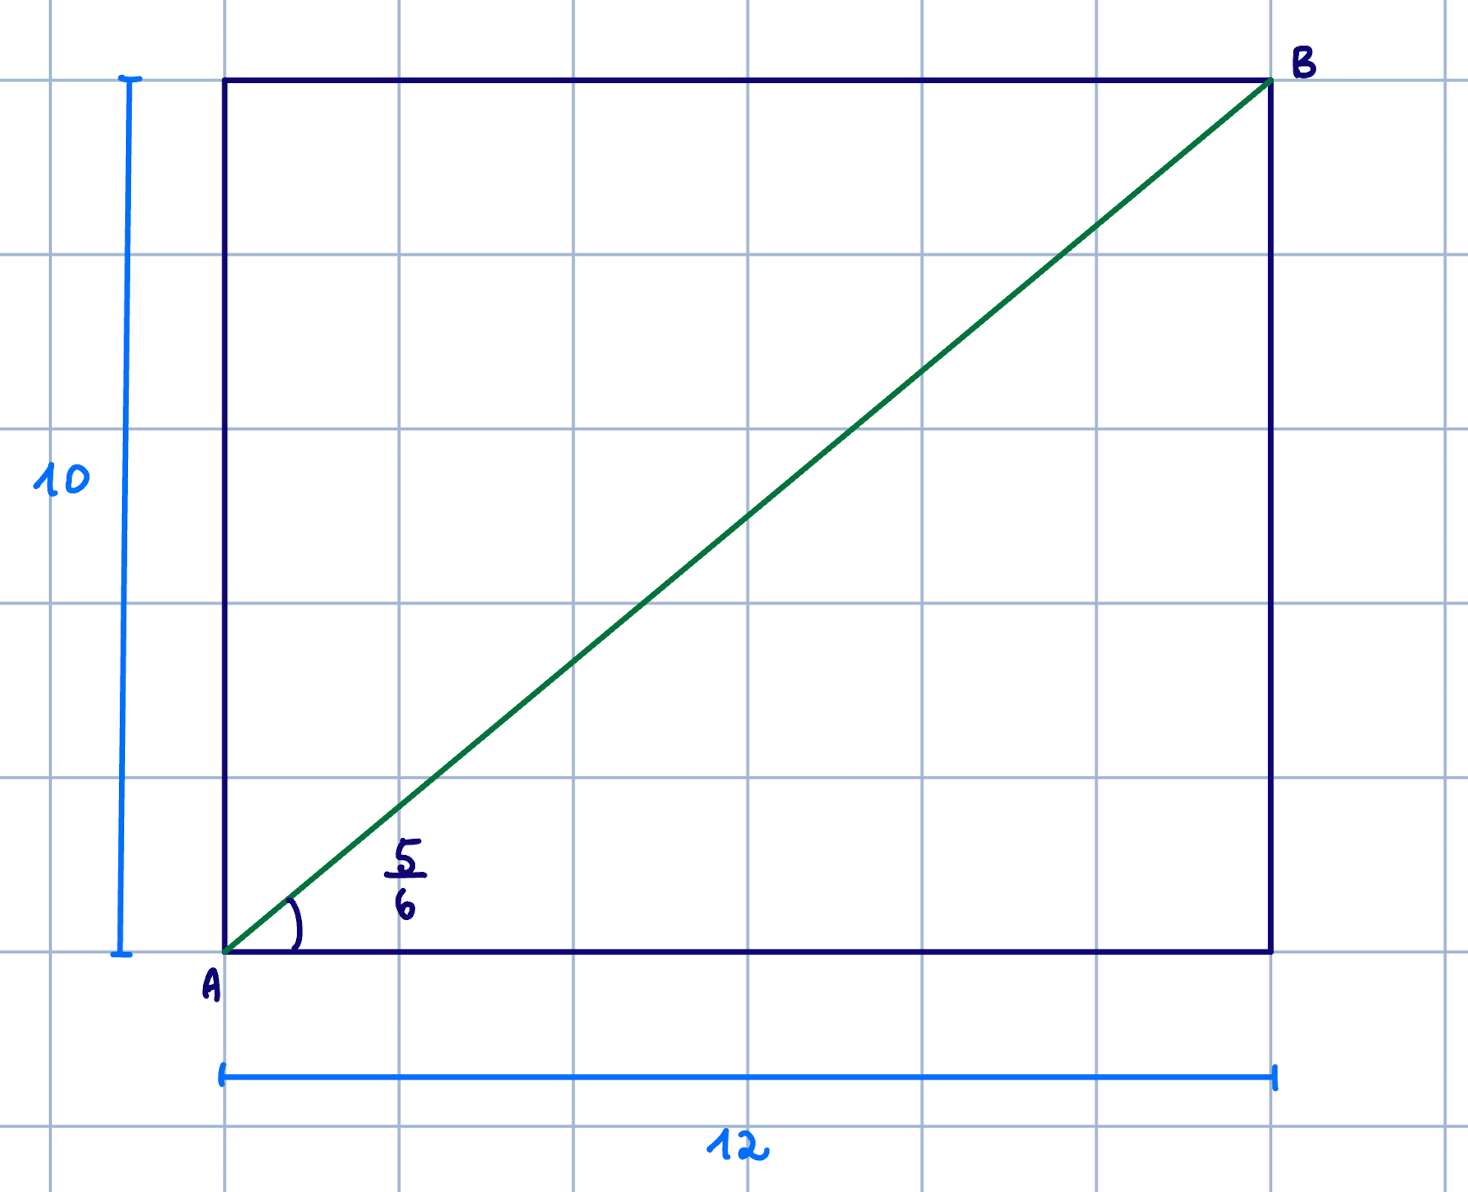
\includegraphics[width=8cm]{fig5.png}
    \caption{Edgeworth Box}
    \label{fig:galaxy}
\end{figure}
\item In the case of perfect complements, we find the contract curve as follows:
\[x_A=6y_A \implies y_A=\frac{5x_A}{6}\]
\[x_B=6y_B \implies y_B=\frac{5x_B}{6}\]
\begin{figure}[H]
    \centering
    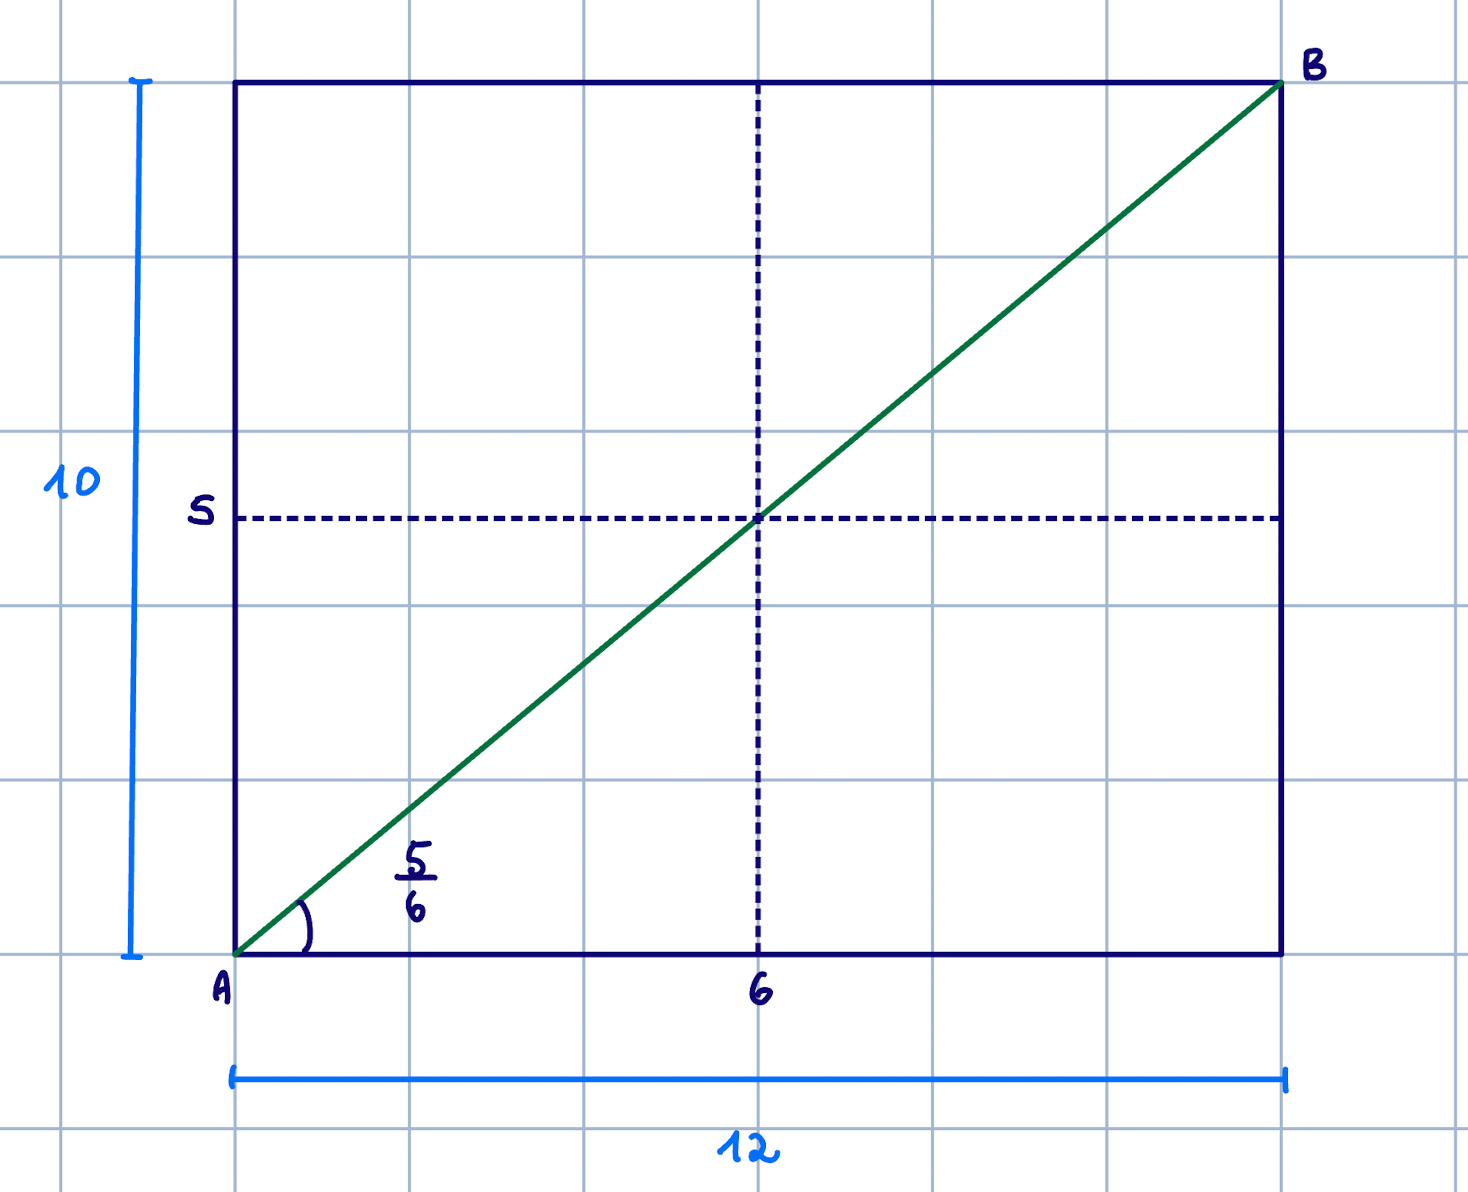
\includegraphics[width=8cm]{fig6.png}
    \caption{Edgeworth Box}
    \label{fig:galaxy}
\end{figure}

\item This is another case of perfect complements:
\[x_A=y_A \qquad and \qquad x_B=y_B\]
\begin{figure}[H]
    \centering
    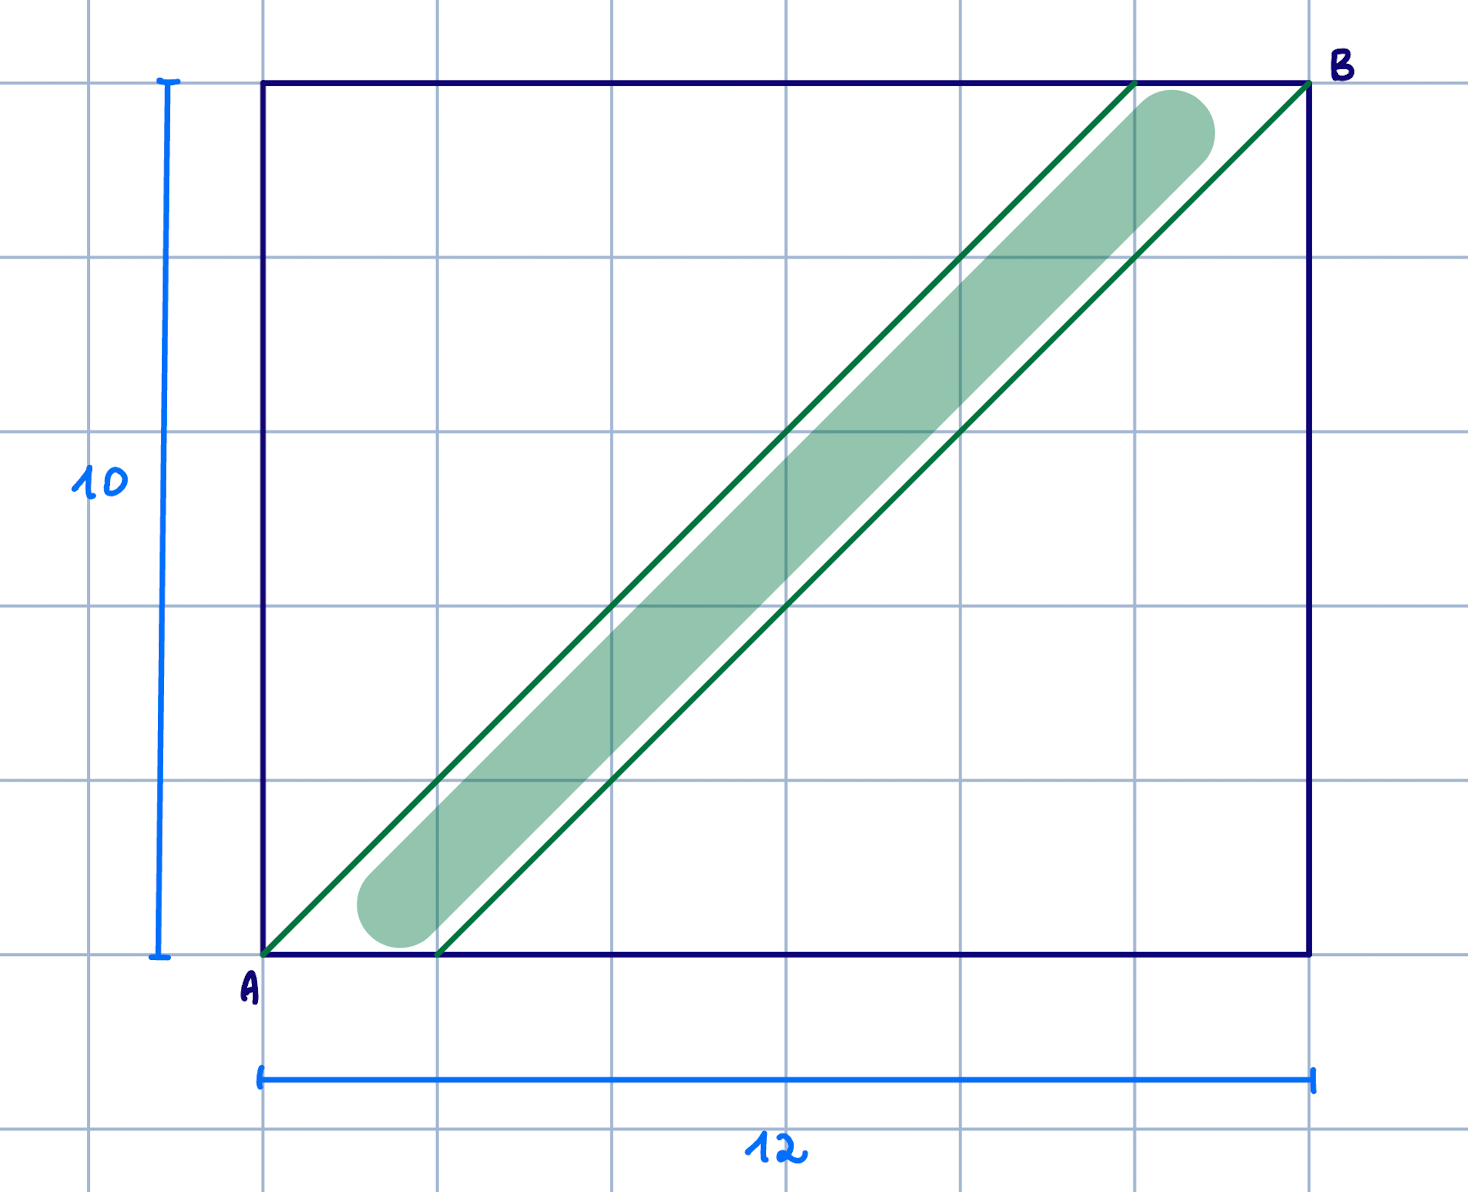
\includegraphics[width=8cm]{fig7.png}
    \caption{Edgeworth Box}
    \label{fig:galaxy}
\end{figure}

\item In the case of perfect substitutes, the contract curve is the following: 

\begin{figure}[H]
    \centering
    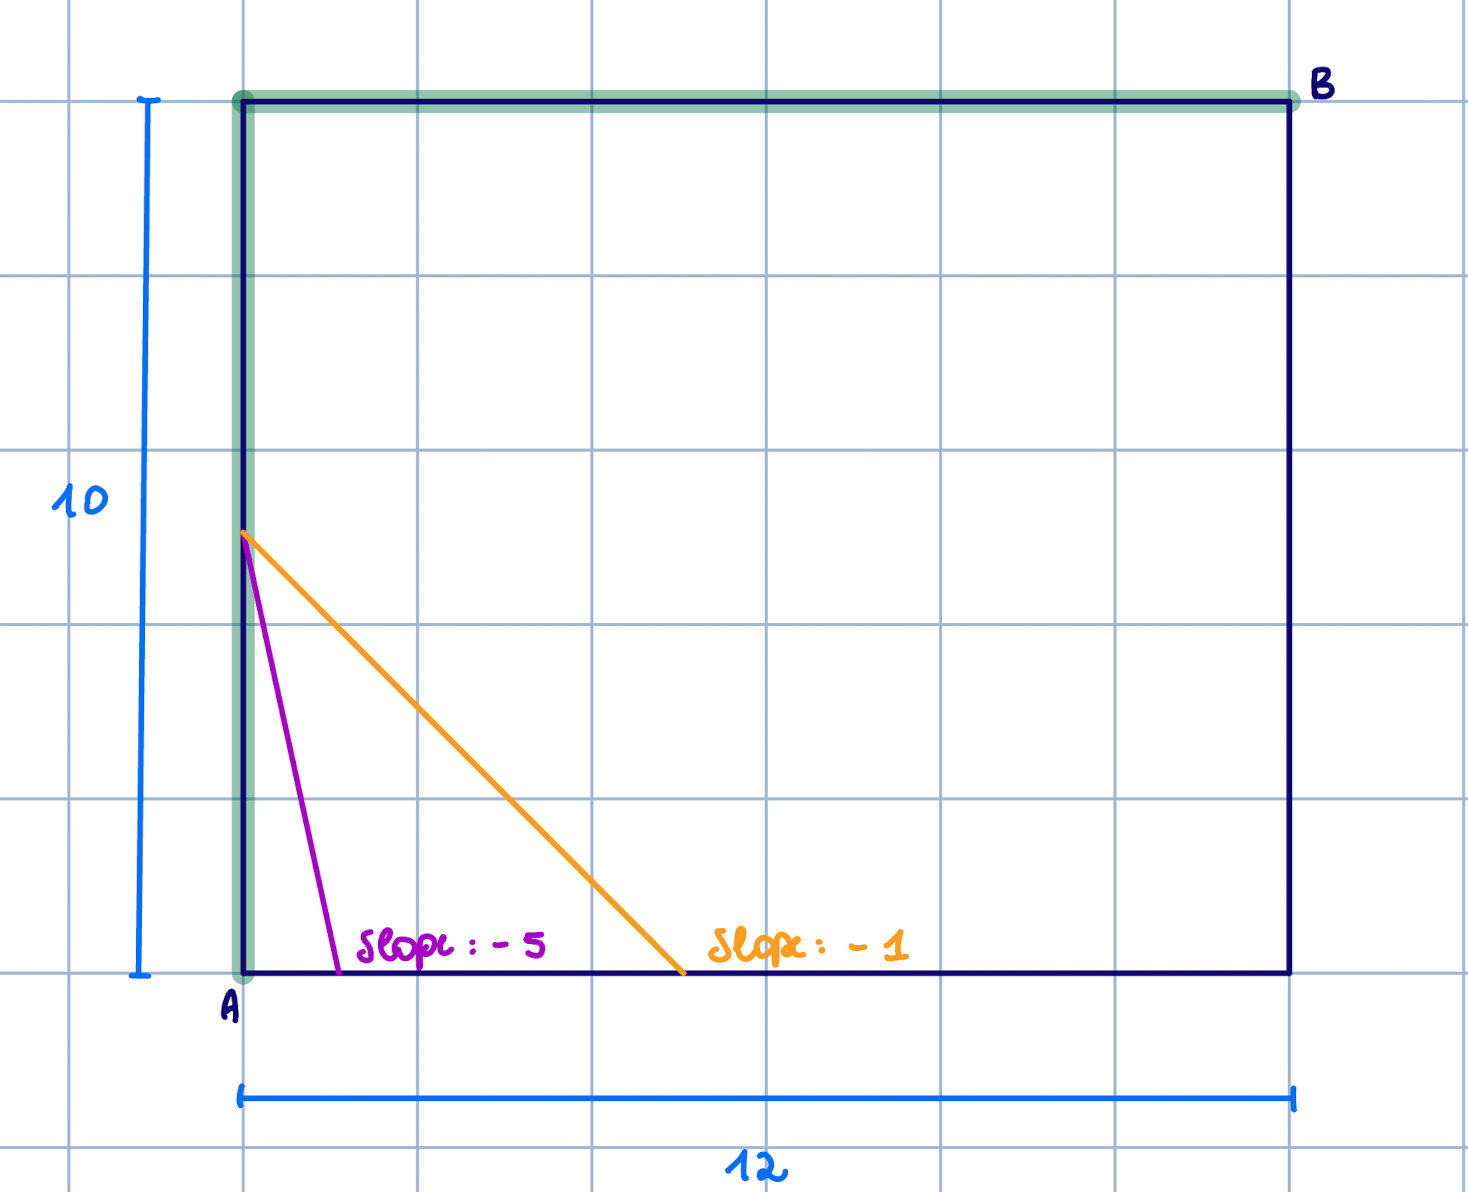
\includegraphics[width=8cm]{fig8.png}
    \caption{Edgeworth Box}
    \label{fig:galaxy}
\end{figure}
\item 
Using the tangency condition and the budget constraint, we obtain:
\[\frac{y_A}{2x_A}=\frac{p_x}{p_y}=\frac{5}{12}\]
The equilibrium price is:
\[\frac{p_x}{p_y}=\frac{5}{12}\]
The optimal consumption bundles are:
\[(x_A^*, y_A^*)=(\frac{74}{15},\frac{37}{9})\]
\[(x_B^*, y_B^*)=(\frac{106}{15},\frac{53}{9})\]
\item In this case, several prices support an equilibrium. That is, as long as there is a price line that passes through the endowment and the point where the two utility functions are "tangent", trade can happen and there is an equilibrium. Therefore, we have multiple equilibrium prices and multiple optimal consumption bundles.
\begin{figure}[H]
    \centering
    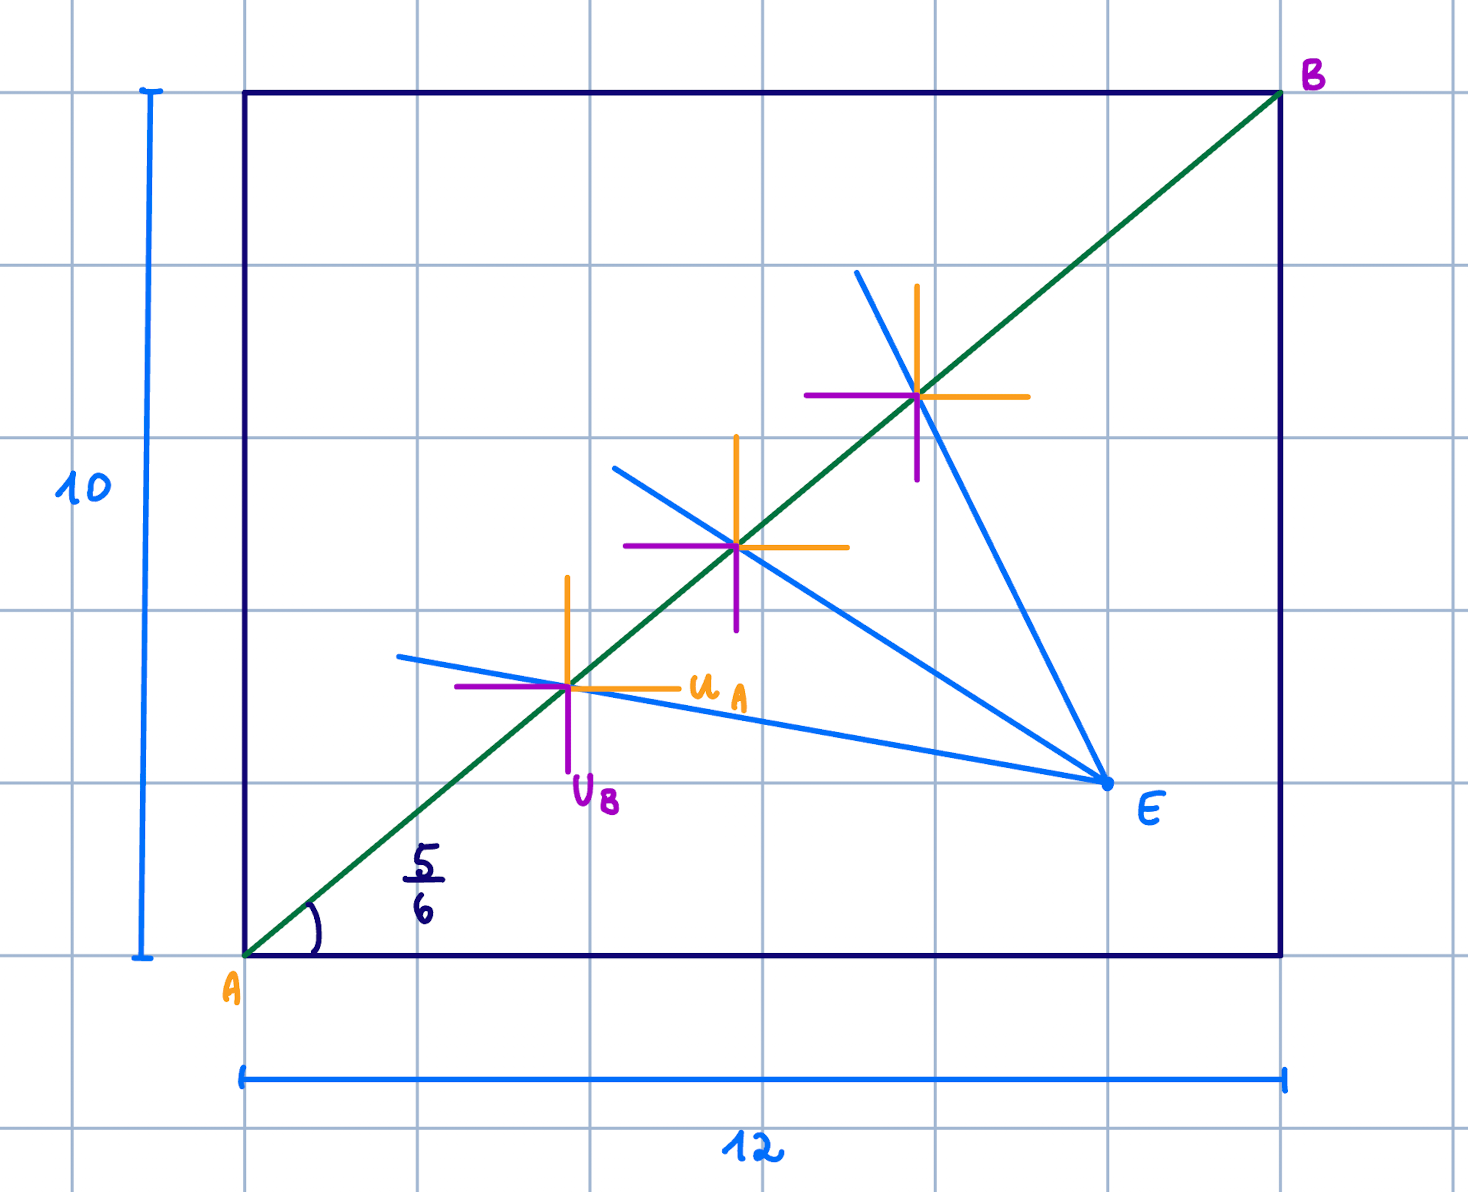
\includegraphics[width=8cm]{fig9.png}
    \caption{Edgeworth Box}
    \label{fig:galaxy}
\end{figure}

\end{enumerate}
\end{document}
